% Brand guide from https://www.kassersynths.com/
% Palette: magenta #ff02ff, cyan #00edff, gold #f1c034 on near-black
% Fonts: Spartan (headings) + Oxanium (body) via fontspec when using XeLaTeX/LuaLaTeX
\documentclass[aspectratio=169,11pt]{beamer}

\usepackage[english]{babel}
\usepackage{iftex}
\ifPDFTeX
  \usepackage[utf8]{inputenc}
  \usepackage[T1]{fontenc}
  \usepackage{lmodern}
\else
  \usepackage{fontspec}
  % League Spartan approximates Google Font ``Spartan'' on the site
  \setsansfont{LeagueSpartan}[
    Path = assets/fonts/,
    UprightFont = *-Regular.ttf,
    BoldFont = *-Bold.ttf,
    ItalicFont = *-Regular.ttf,
    BoldItalicFont = *-Bold.ttf,
    Ligatures = TeX
  ]
  \setmainfont{Oxanium}[
    Path = assets/fonts/,
    UprightFont = *-Regular.ttf,
    BoldFont = *-Bold.ttf,
    ItalicFont = *-Regular.ttf,
    BoldItalicFont = *-Bold.ttf,
    Ligatures = TeX
  ]
  \renewcommand{\familydefault}{\rmdefault}
\fi
\usepackage{booktabs}
\usepackage{graphicx}
\usepackage{hyperref}
\usepackage{tikz}
\usepackage{xcolor}

% ===== Kasser Synths brand (site palette) =====
\definecolor{kasserMagenta}{HTML}{FF02FF}
\definecolor{kasserCyan}{HTML}{00EDFF}
\definecolor{kasserGold}{HTML}{F1C034}
\definecolor{kasserBlue}{HTML}{0089F7}
\definecolor{kasserBlack}{HTML}{0A0A0A}
\definecolor{kasserPanel}{HTML}{161922}
\definecolor{kasserMuted}{HTML}{929292}
\definecolor{kasserGray}{HTML}{444444}

\usetheme{Madrid}
\usecolortheme{default}

\setbeamercolor{normal text}{fg=white,bg=kasserBlack}
\setbeamercolor{background canvas}{bg=kasserBlack}
\setbeamercolor{structure}{fg=kasserMagenta}
\setbeamercolor{titlelike}{fg=white}
\setbeamercolor{title}{fg=white,bg=kasserPanel}
\setbeamercolor{subtitle}{fg=kasserCyan}
\setbeamercolor{frametitle}{fg=white,bg=kasserPanel}
\setbeamercolor{block title}{fg=kasserBlack,bg=kasserMagenta}
\setbeamercolor{block body}{fg=white,bg=kasserPanel}
\setbeamercolor{block title alerted}{fg=kasserBlack,bg=kasserGold}
\setbeamercolor{block body alerted}{fg=white,bg=kasserPanel}
\setbeamercolor{author in head/foot}{bg=kasserMagenta,fg=kasserBlack}
\setbeamercolor{title in head/foot}{bg=kasserPanel,fg=white}
\setbeamercolor{date in head/foot}{bg=kasserCyan,fg=kasserBlack}
\setbeamercolor{itemize item}{fg=kasserCyan}
\setbeamercolor{itemize subitem}{fg=kasserMagenta}
\setbeamercolor{enumerate item}{fg=kasserCyan}

\ifPDFTeX
  \setbeamerfont{frametitle}{series=\bfseries,size=\Large}
  \setbeamerfont{title}{series=\bfseries,size=\LARGE}
  \setbeamerfont{block title}{series=\bfseries}
\else
  \setbeamerfont{normal text}{family=\rmfamily}
  \setbeamerfont{frametitle}{family=\sffamily,series=\bfseries,size=\Large}
  \setbeamerfont{title}{family=\sffamily,series=\bfseries,size=\LARGE}
  \setbeamerfont{subtitle}{family=\rmfamily,size=\large}
  \setbeamerfont{author}{family=\rmfamily}
  \setbeamerfont{institute}{family=\rmfamily,size=\small}
  \setbeamerfont{block title}{family=\sffamily,series=\bfseries}
\fi

\setbeamertemplate{navigation symbols}{}
\setbeamertemplate{itemize item}{\color{kasserCyan}\small$\blacktriangleright$}
\setbeamertemplate{itemize subitem}{\color{kasserMagenta}\tiny$\bullet$}

\hypersetup{colorlinks=true,linkcolor=kasserCyan,urlcolor=kasserCyan,citecolor=kasserGold}

\newcommand{\videobox}[2]{%
  \begin{center}
    \fcolorbox{kasserMagenta}{kasserPanel}{%
      \parbox{0.92\linewidth}{%
        \centering\vspace{2.5mm}
        {\large\color{kasserMagenta}\textbf{$\blacktriangleright$ VIDEO #1}}\\[1.5mm]
        {\small\color{white}#2}\\[1mm]
        {\scriptsize\color{kasserMuted}\textit{Placeholder --- replace with \texttt{videos/V#1.mp4}}}
        \vspace{2.5mm}
      }%
    }
  \end{center}
}

\newcommand{\livebox}[2]{%
  \vspace{1mm}
  \begin{center}
    \fcolorbox{kasserGold}{kasserPanel}{%
      \parbox{0.94\linewidth}{%
        \centering\vspace{1mm}
        {\small\color{kasserGold}\textbf{$\blacktriangleright$ LIVE #1}}~~
        {\scriptsize\color{white}#2}\\[0.5mm]
        {\tiny\color{kasserMuted}\textit{\texttt{videos/LIVE\_DEMOS.md}}}
        \vspace{1mm}
      }%
    }
  \end{center}
}

\newcommand{\photoplaceholder}[1]{%
  \fcolorbox{kasserCyan}{kasserPanel}{%
    \parbox[c][2.8cm][c]{0.92\linewidth}{%
      \centering\color{kasserMuted}\scriptsize\textit{Photo placeholder}\\[1mm]\texttt{#1}%
    }%
  }%
}

\title[DAFMExplorer @ Ludo2026]{Exploring the Sonic Universe of the Sega Genesis}
\subtitle{Data Science, FM Synthesis, and 93{,}000+ Presets}
\author[Casas \& Cerro]{%
  Abraham Casas\\\small Electronics \& CTO, Kasser Synths
  \and
  Maria Cerro\\\small Design \& CEO, Kasser Synths}
\institute[Kasser Synths]{Kasser Synths\\[1mm]{\scriptsize Ludo2026 --- Session 9: \textit{Synthesis, Served Three Ways}}}
\date{August 2026}
\titlegraphic{%
  \IfFileExists{assets/logo-kasser-synths.png}{%
    
\includegraphics[height=1.05cm,keepaspectratio]{assets/logo-kasser-synths.png}%
  }{%
    \IfFileExists{assets/logo-kasser-synths.svg}{%
      
\includegraphics[height=1.05cm,keepaspectratio]{assets/logo-kasser-synths.svg}%
    }{}%
  }%
}

\begin{document}

%---------------------------------------------------------------------
\begin{frame}
  \titlepage
\end{frame}

%---------------------------------------------------------------------
\begin{frame}{Who we are}
  \begin{columns}[T,onlytextwidth]
    \column{0.48\textwidth}
    \centering
    \IfFileExists{assets/photo_abraham.png}{%
      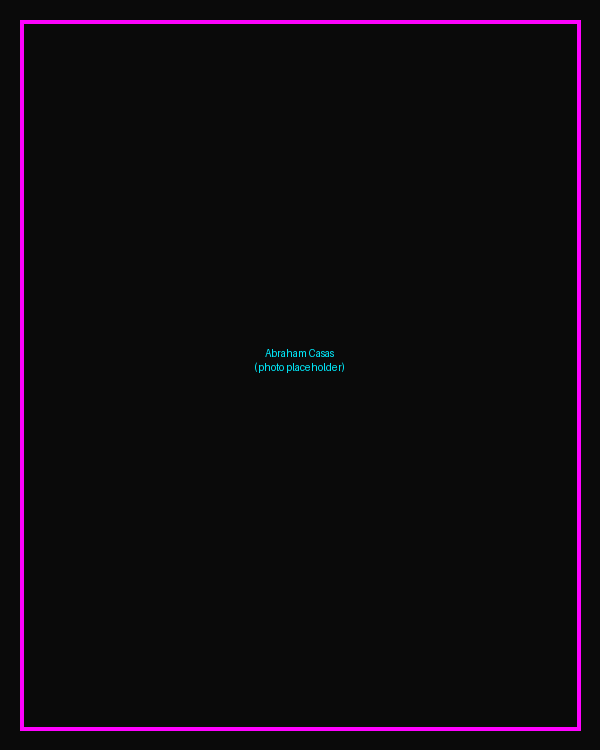
\includegraphics[height=2.8cm,keepaspectratio]{assets/photo_abraham.png}%
    }{\photoplaceholder{assets/photo\_abraham.png}}
    \vspace{1mm}

    \textbf{Abraham Casas}\\
    {\small Electronics \& CTO}\\
    {\scriptsize Presenting today}
    \column{0.48\textwidth}
    \centering
    \IfFileExists{assets/photo_maria.png}{%
      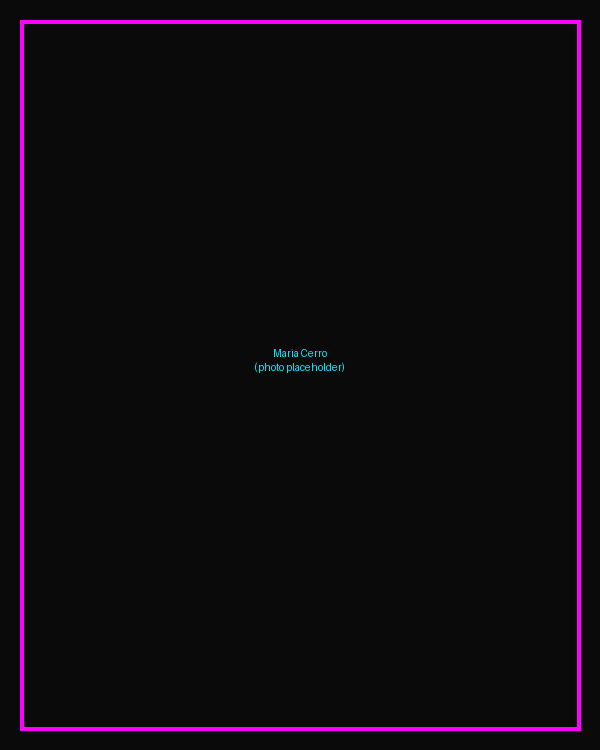
\includegraphics[height=2.8cm,keepaspectratio]{assets/photo_maria.png}%
    }{\photoplaceholder{assets/photo\_maria.png}}
    \vspace{1mm}

    \textbf{Maria Cerro}\\
    {\small Design \& CEO}
  \end{columns}
  \vspace{2mm}
  \begin{block}{Kasser Synths}
    A small studio exploring Yamaha FM chips and the sonic legacy of 1980s--90s games.\\
    \textbf{DAFMExplorer} is our open project for reading that legacy as structured data --- and listening to it again.
  \end{block}
\end{frame}

%---------------------------------------------------------------------
\begin{frame}{A platform's voice is also its presets}
  \begin{columns}[c,onlytextwidth]
    \column{0.48\textwidth}
    \IfFileExists{assets/Sega-Genesis-Mod1-Bare.jpg}{%
      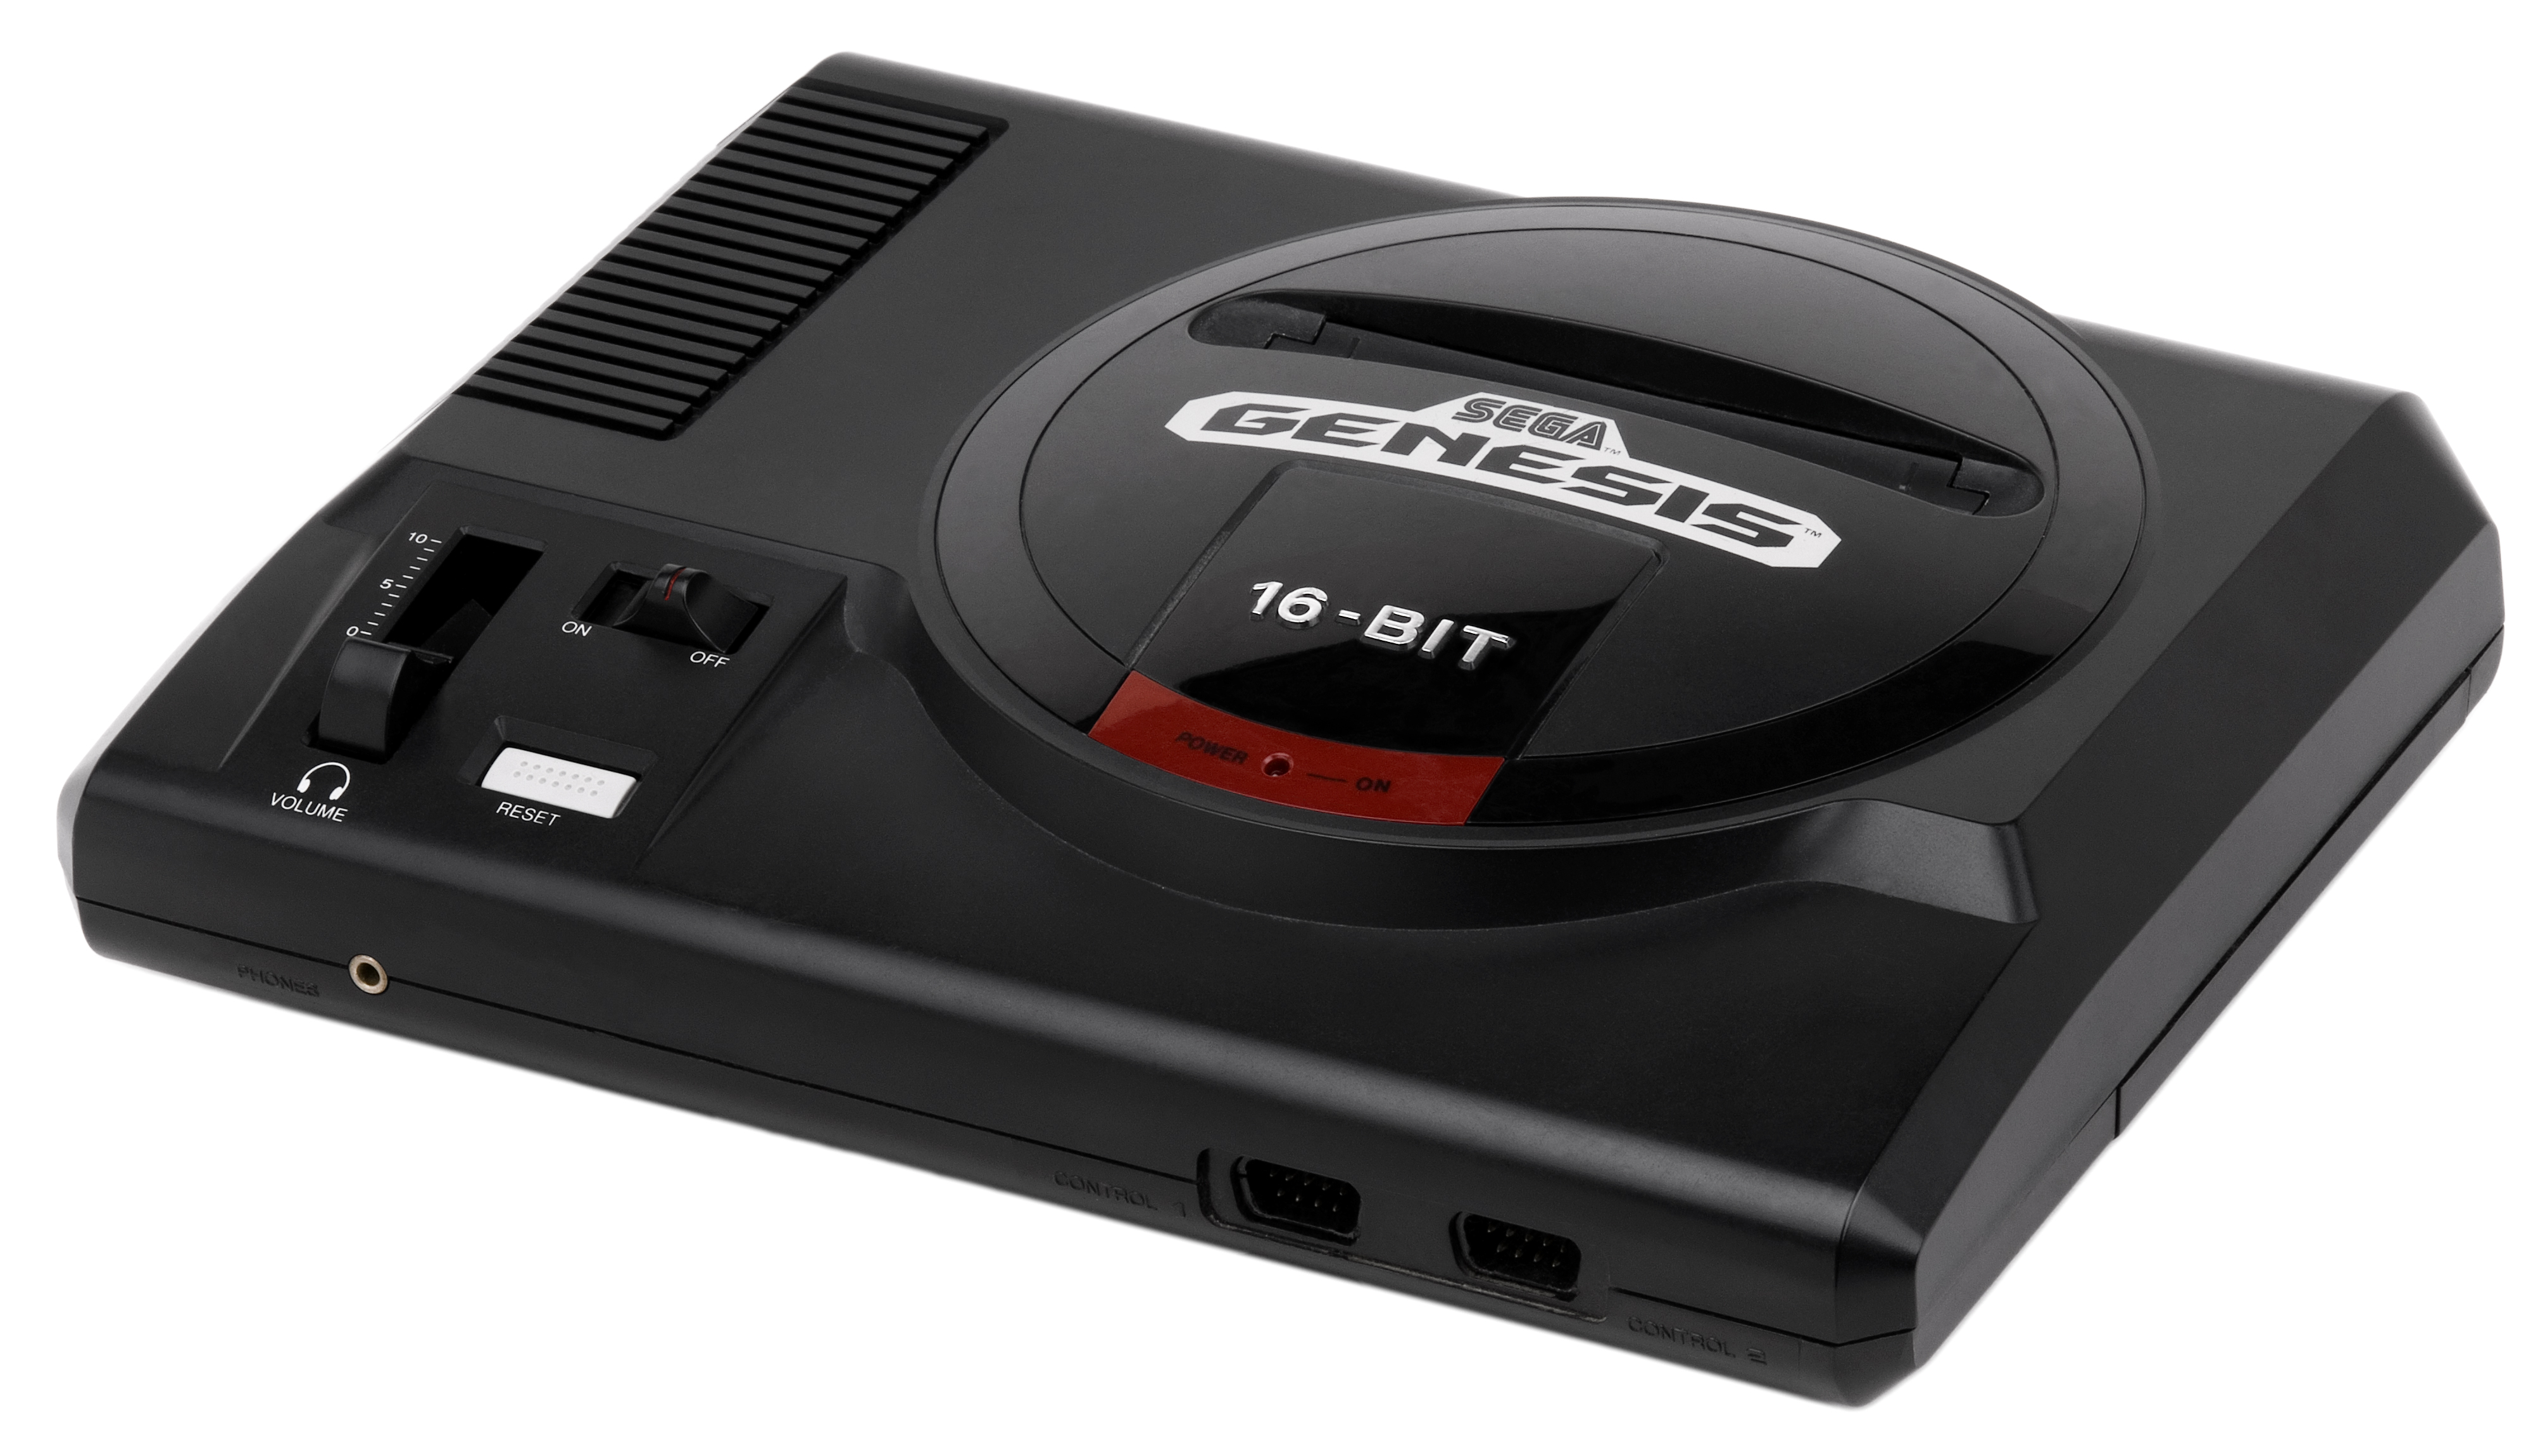
\includegraphics[width=\linewidth,height=0.55\textheight,keepaspectratio]{assets/Sega-Genesis-Mod1-Bare.jpg}%
    }{}
    \column{0.50\textwidth}
    Beyond melodies and arrangements, Genesis music is built from \textbf{programmed FM timbres}:
    \begin{itemize}
      \item Reused across tracks and scenes
      \item Tuned for tiny TV speakers
      \item Authored under the constraints of one chip
    \end{itemize}
    \vspace{2mm}
    {\small Those presets are creative decisions --- and historical evidence.}
  \end{columns}
\end{frame}

%---------------------------------------------------------------------
\begin{frame}{From Chowning to the living room}
  \begin{columns}[T,onlytextwidth]
    \column{0.32\textwidth}
    \centering
    \IfFileExists{assets/John-Chowning-Stanford.jpg}{%
      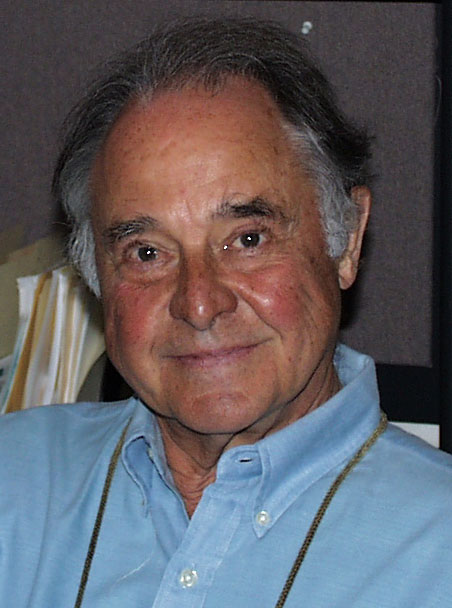
\includegraphics[width=\linewidth,height=0.38\textheight,keepaspectratio]{assets/John-Chowning-Stanford.jpg}%
    }{}
    \vspace{1mm}\\{\scriptsize Chowning / CCRMA}
    \column{0.32\textwidth}
    \centering
    \IfFileExists{assets/Yamaha-DX7.jpg}{%
      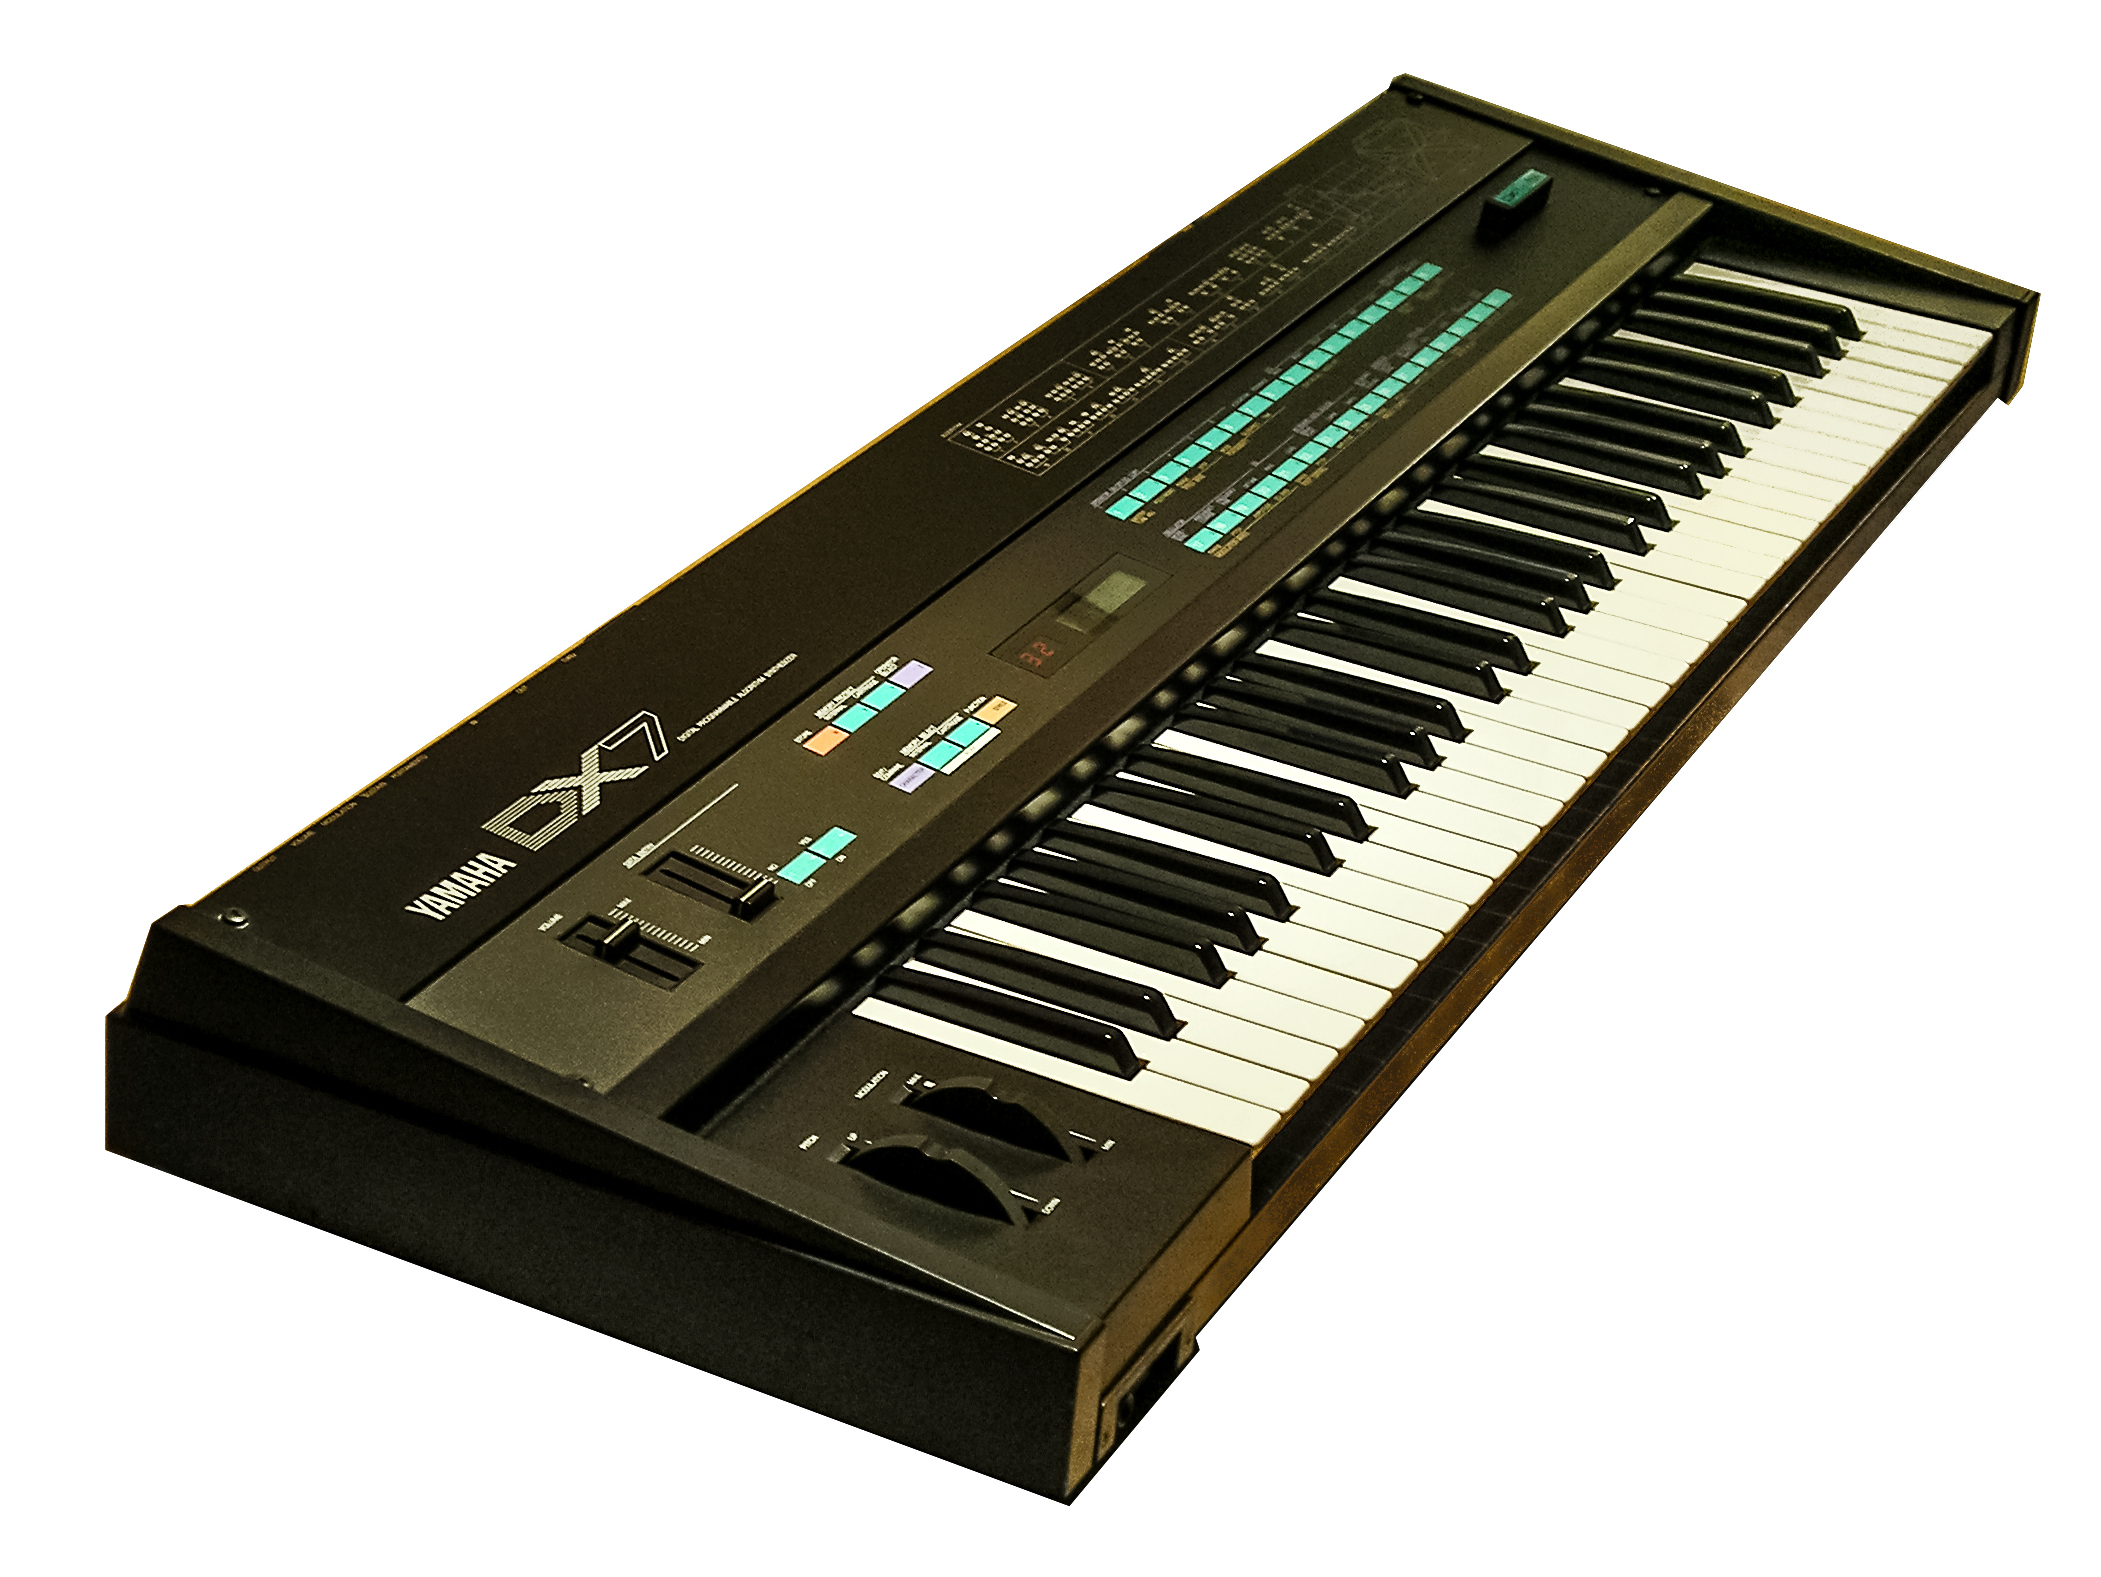
\includegraphics[width=\linewidth,height=0.38\textheight,keepaspectratio]{assets/Yamaha-DX7.jpg}%
    }{}
    \vspace{1mm}\\{\scriptsize Yamaha DX7 (6 ops)}
    \column{0.32\textwidth}
    \centering
    \IfFileExists{assets/YM2612-chip.jpg}{%
      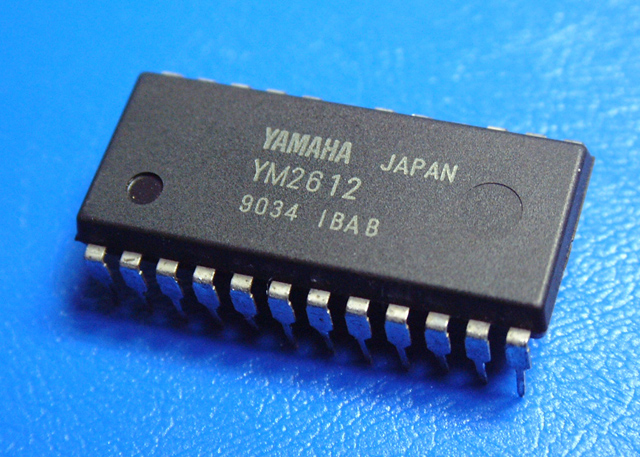
\includegraphics[width=\linewidth,height=0.38\textheight,keepaspectratio]{assets/YM2612-chip.jpg}%
    }{}
    \vspace{1mm}\\{\scriptsize YM2612: \textbf{4 ops, 8 algorithms}}
  \end{columns}
  \vspace{3mm}
  Same mathematical idea --- frequency modulation --- different creative solutions on every game.
\end{frame}

%---------------------------------------------------------------------
\begin{frame}{The underexplored archive}
  \begin{columns}[T,onlytextwidth]
    \column{0.55\textwidth}
    \begin{itemize}
      \item \textbf{VGM}: exact chip-command recordings
      \item \textbf{Project2612} / VGMrips: preservation at scale
      \item \textbf{DrWashington} collection: OPM presets extracted from those VGMs
    \end{itemize}
    \vspace{2mm}
    \begin{alertblock}{93{,}000+ presets}
      A huge corpus of YM2612 voices --- still underexplored as \textbf{structured data} in ludomusicology.
    \end{alertblock}
    \column{0.42\textwidth}
    \centering
    \IfFileExists{assets/project2612-logo.png}{%
      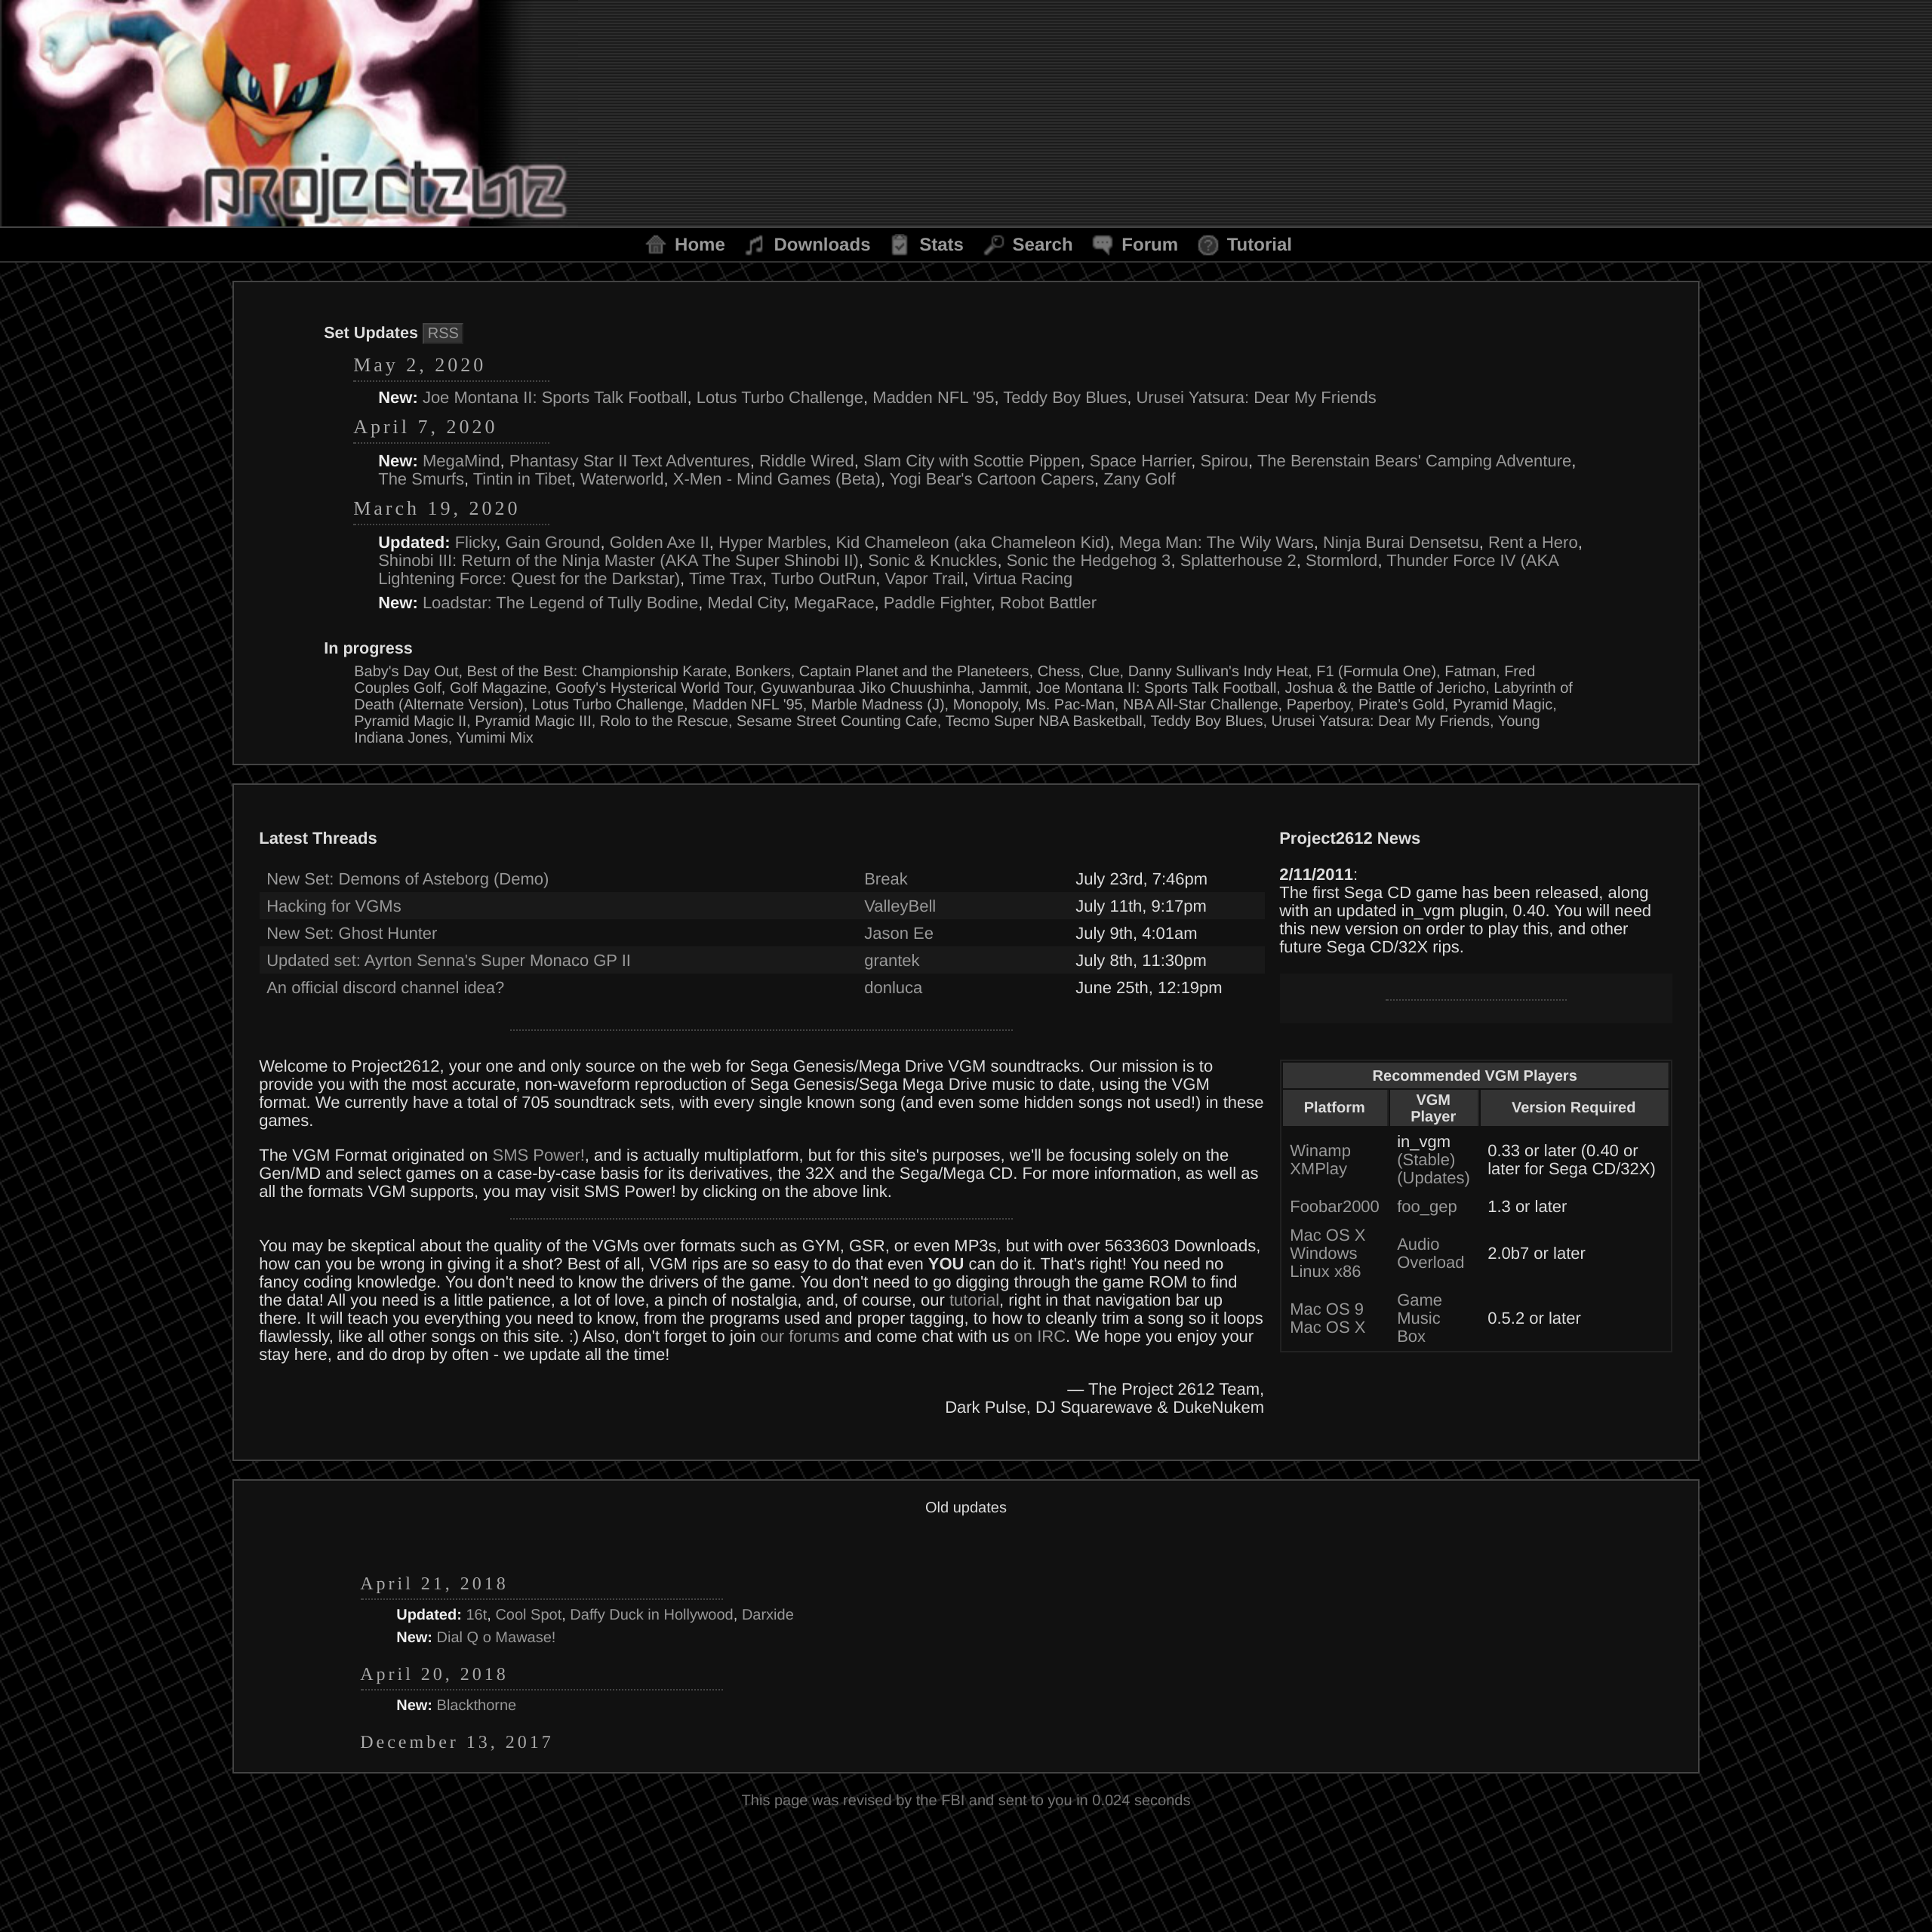
\includegraphics[width=0.85\linewidth,height=0.22\textheight,keepaspectratio]{assets/project2612-logo.png}%
    }{}
    \vspace{2mm}
    \IfFileExists{assets/vgmrips-website.png}{%
      
\includegraphics[width=0.95\linewidth,height=0.28\textheight,keepaspectratio]{assets/vgmrips-website.png}%
    }{}
  \end{columns}
\end{frame}

%---------------------------------------------------------------------
\begin{frame}{Live listening kit --- games, music, presets}
  Four short live moments (VGM track $\rightarrow$ related preset). Keep each under $\sim$20--25\,s.
  \vspace{1mm}
  {\scriptsize
  \begin{tabular}{@{}clll@{}}
  \toprule
  \textbf{\#} & \textbf{Game} & \textbf{Hear in the music} & \textbf{Then isolate a preset} \\
  \midrule
  L1 & \textit{Streets of Rage} & Koshiro's club energy & high-feedback lead / bass \\
  L2 & \textit{Pulseman} & one-topology brand & Alg.~5 bright patch \\
  L3 & \textit{Nightmare Circus} & GEMS-era US title & tool-shaped voice \\
  L4 & \textit{Thunder Force IV} & dense shoot-'em-up FM & varied CON neighbour \\
  \bottomrule
  \end{tabular}
  }
  \vspace{2mm}
  \begin{columns}[T,onlytextwidth]
    \column{0.48\textwidth}
    \begin{block}{VGM (offline)}
      {\small Foobar2000 + in\_vgm, or VGMPlay --- files from VGMrips, cached on the laptop.}
    \end{block}
    \column{0.48\textwidth}
    \begin{block}{Preset (live)}
      {\small DAFMExplorer filter by game $\rightarrow$ click $\rightarrow$ play YM2612.\\
      {\scriptsize\url{https://dafm-explorer.vercel.app/}}}
    \end{block}
  \end{columns}
\end{frame}

%---------------------------------------------------------------------
\begin{frame}{Data extraction --- Making the archive speak}
  Turning raw OPM into an analysis-ready corpus:
  \begin{enumerate}
    \item Parse presets (channel + 4 operators $\approx$ 58 parameters)
    \item Deduplicate by timbre (ignore \textbf{TL} volume variants --- same voice, different mix level)
    \item Normalise game names (regional titles, aliases)
    \item Enrich: composer, nationality, \textbf{GEMS} usage (Sega Retro, VGMrips, Wikipedia)
  \end{enumerate}
  \videobox{1}{From OPM file $\rightarrow$ a named preset with game, composer, and tool metadata}
\end{frame}

%---------------------------------------------------------------------
\begin{frame}{Why TL breaks naive counting}
  \begin{columns}[c,onlytextwidth]
    \column{0.58\textwidth}
    \IfFileExists{assets/fig_tl_dedup.png}{%
      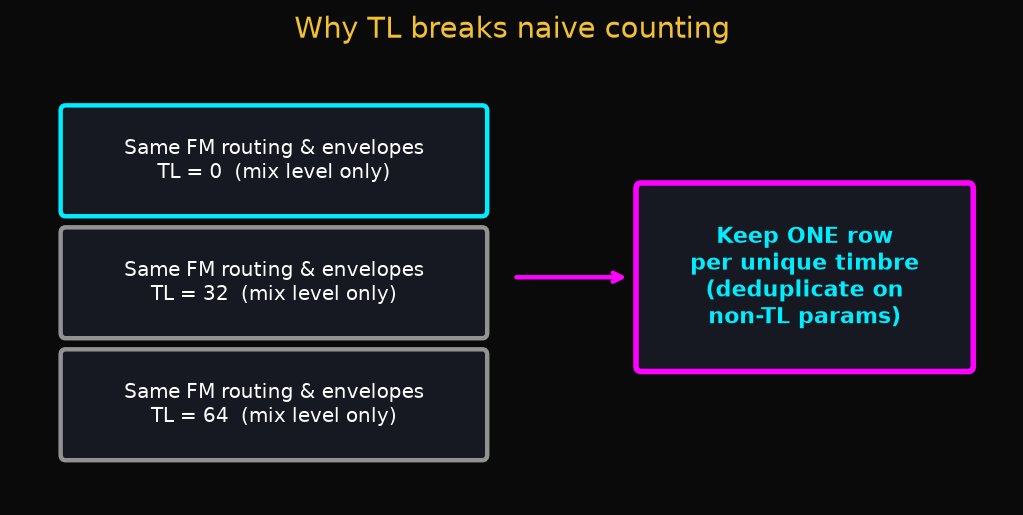
\includegraphics[width=\linewidth]{assets/fig_tl_dedup.png}%
    }{}
    \column{0.40\textwidth}
    Games reuse the same patch at different mix levels.
    \begin{itemize}
      \item \textbf{TL} = loudness in the arrangement, not a new timbre
      \item Counting every row would invent thousands of ``fake'' instruments
      \item Dedup on non-TL parameters keeps the creative decision once
    \end{itemize}
  \end{columns}
\end{frame}

%---------------------------------------------------------------------
\begin{frame}{What an FM preset is}
  \begin{columns}[T,onlytextwidth]
    \column{0.52\textwidth}
    \textbf{Channel}
    \begin{itemize}
      \item \textbf{CON} --- algorithm (how operators connect)
      \item \textbf{FL} --- feedback on operator~1
      \item Pan, LFO, \ldots
    \end{itemize}
    \vspace{2mm}
    \textbf{Four operators} (M1, C1, M2, C2)
    \begin{itemize}
      \item Envelopes (AR, D1R, D2R, RR, \ldots)
      \item \textbf{TL} --- level / mix
      \item \textbf{MUL} --- frequency ratio
    \end{itemize}
    \column{0.45\textwidth}
    \IfFileExists{assets/opm-file-example.png}{%
      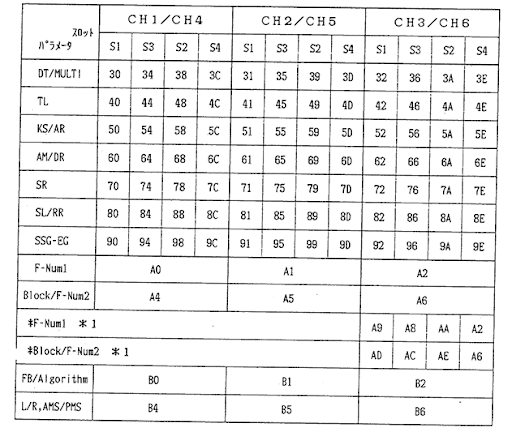
\includegraphics[width=\linewidth,height=0.55\textheight,keepaspectratio]{assets/opm-file-example.png}%
    }{}
  \end{columns}
  \vspace{1mm}
  {\small Carriers you hear; modulators shape their spectrum. Each preset = a creative solution under chip constraints.}
\end{frame}

%---------------------------------------------------------------------
\begin{frame}{Algorithms as wiring diagrams}
  \begin{center}
    \IfFileExists{assets/fig_algorithms_schematic.png}{%
      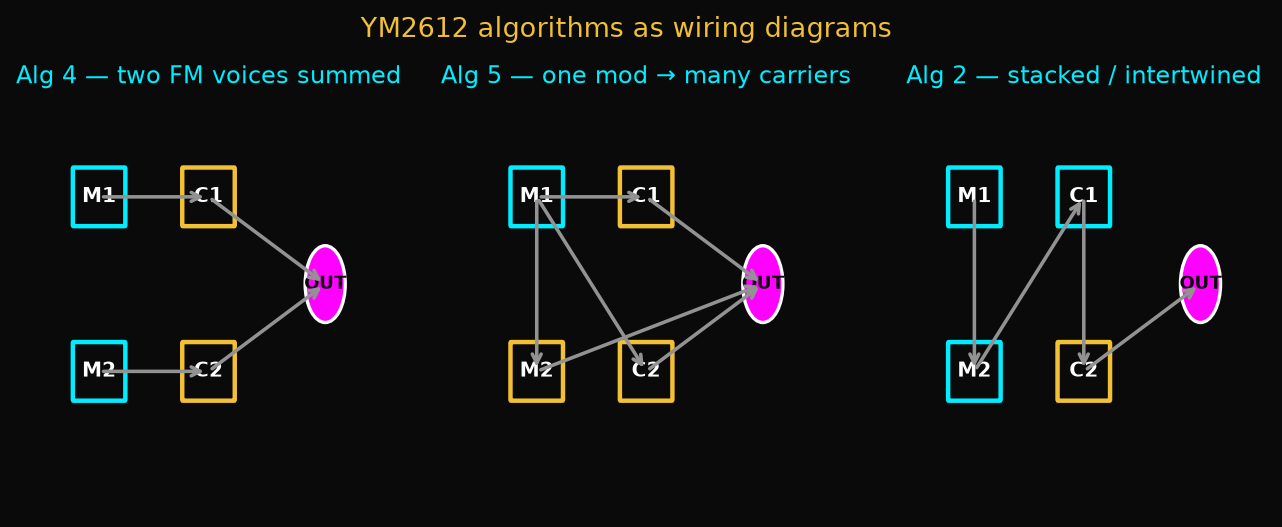
\includegraphics[width=0.98\linewidth,height=0.58\textheight,keepaspectratio]{assets/fig_algorithms_schematic.png}%
    }{}
  \end{center}
  \vspace{1mm}
  {\small Same four operators; different \textbf{CON} = different instrument architecture. Gold $\approx$ carriers, cyan $\approx$ modulators.}
\end{frame}

%---------------------------------------------------------------------
\begin{frame}{EDA: Algorithm 4 as the workhorse}
  \begin{columns}[c,onlytextwidth]
    \column{0.52\textwidth}
    \IfFileExists{assets/fig_con_distribution.png}{%
      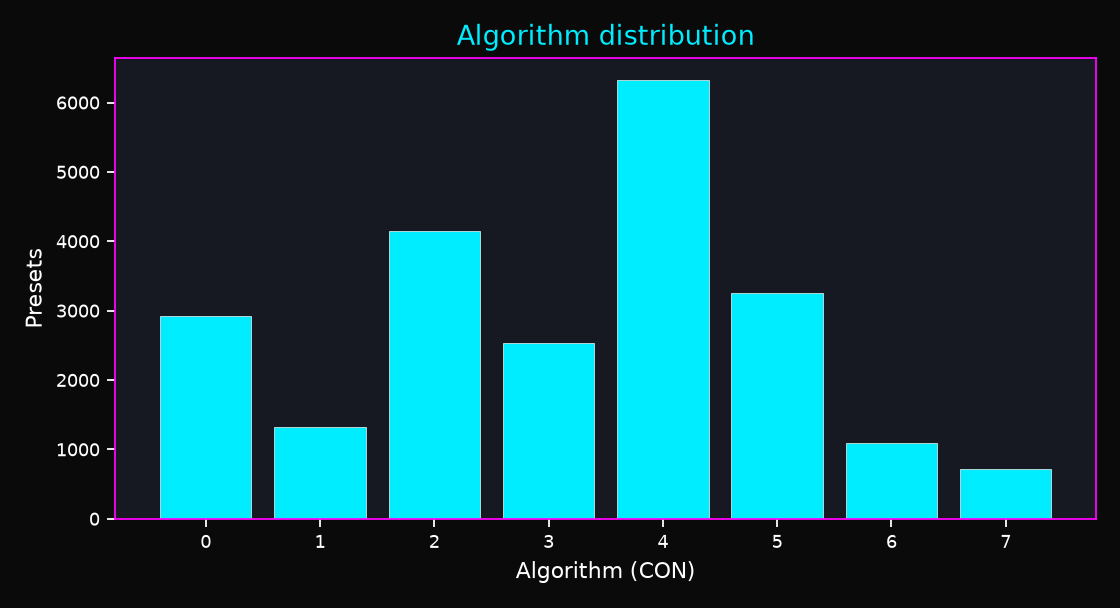
\includegraphics[width=\linewidth]{assets/fig_con_distribution.png}%
    }{%
      \fcolorbox{kasserMagenta}{kasserPanel}{\parbox[c][4cm][c]{\linewidth}{\centering\color{kasserMuted}\scriptsize Export \texttt{fig\_con\_distribution.png}}}%
    }
    \column{0.45\textwidth}
    \begin{itemize}
      \item \textbf{Algorithm 4} dominates corpus-wide: two FM voices summed --- flexible and mix-friendly
      \item Some scores commit hard to one topology
      \item Others spread routing across several algorithms
    \end{itemize}
    \vspace{2mm}
    {\small A shared ``YM2612 grammar'' --- with room for fingerprints.}
  \end{columns}
\end{frame}

%---------------------------------------------------------------------
\begin{frame}{Game fingerprints --- commit vs variety}
  \begin{columns}[c,onlytextwidth]
    \column{0.55\textwidth}
    \IfFileExists{assets/fig_fingerprint_games.png}{%
      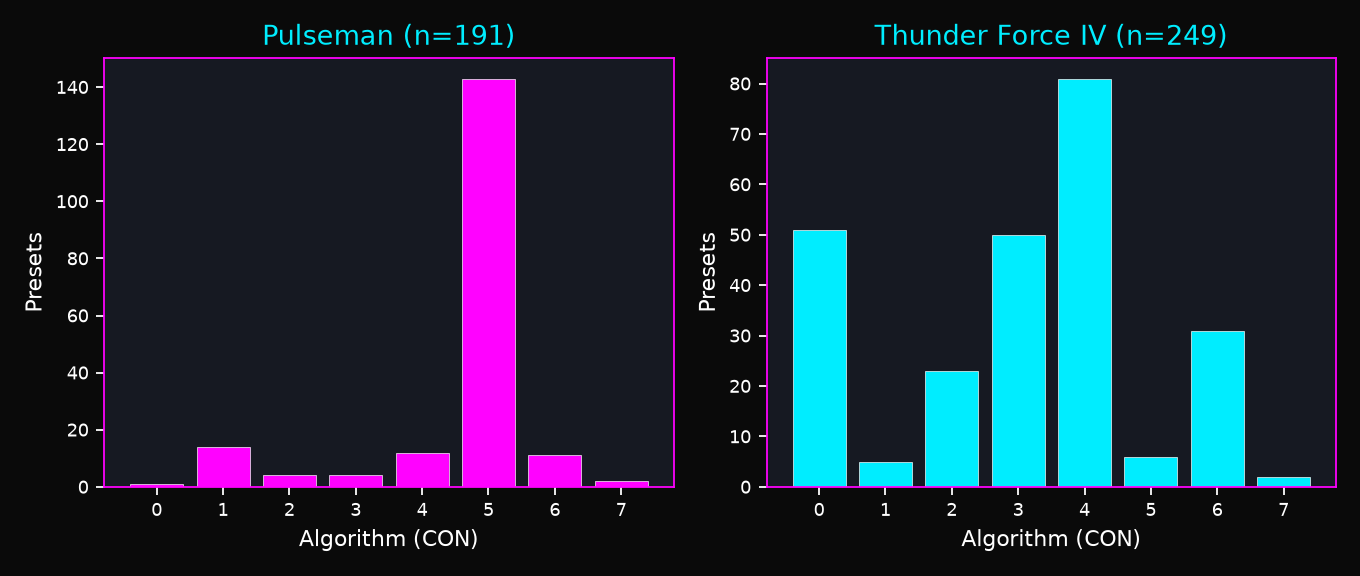
\includegraphics[width=\linewidth,height=0.48\textheight,keepaspectratio]{assets/fig_fingerprint_games.png}%
    }{}
    \column{0.42\textwidth}
    \begin{itemize}
      \item \textbf{Pulseman}: one algorithm dominates (Alg.~5) --- brand by commitment
      \item \textbf{Thunder Force~IV}: spreads across CONs --- identity from variety
    \end{itemize}
    {\scriptsize Same chip, different house styles of sound design.}
  \end{columns}
  \livebox{L2}{\textit{Pulseman} VGM $\rightarrow$ Alg.~5 preset in DAFMExplorer}
\end{frame}

%---------------------------------------------------------------------
\begin{frame}{EDA: Feedback as a binary aesthetic}
  \begin{columns}[c,onlytextwidth]
    \column{0.48\textwidth}
    \IfFileExists{assets/fig_fl_distribution.png}{%
      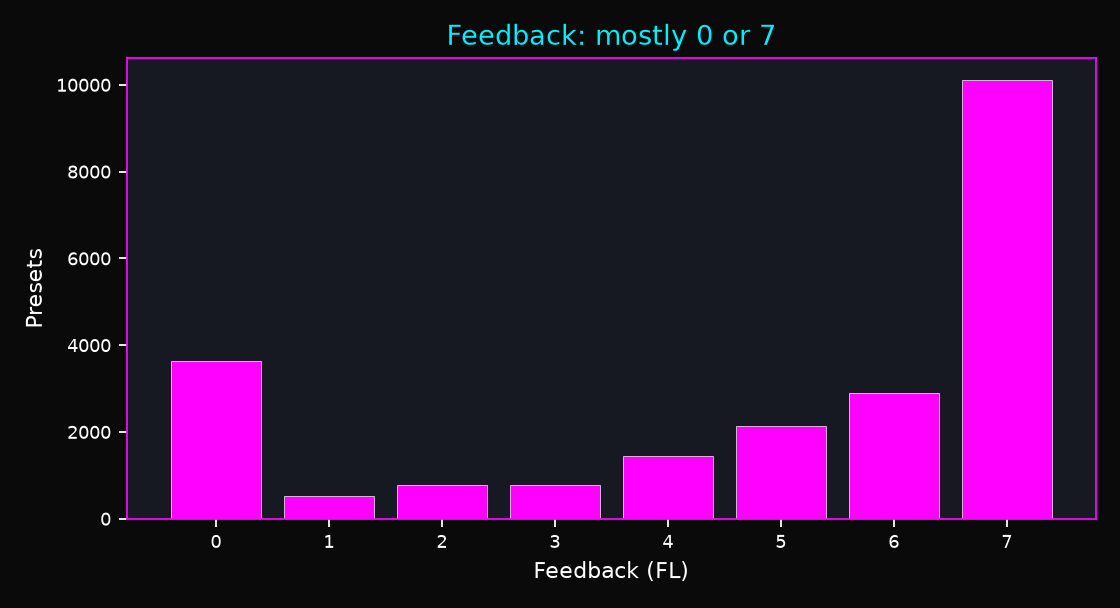
\includegraphics[width=\linewidth,height=0.42\textheight,keepaspectratio]{assets/fig_fl_distribution.png}%
    }{}
    \column{0.50\textwidth}
    Almost no middle ground: \textbf{FL = 0} or \textbf{FL = 7}.
    \begin{itemize}
      \item Max feedback: grit, cut, presence
      \item No feedback: clean, controllable
    \end{itemize}
    {\scriptsize A stylistic switch, not a gentle trim.}
  \end{columns}
  \videobox{2}{Hear FL~0 vs FL~7 (or two extreme presets)}
\end{frame}

%---------------------------------------------------------------------
\begin{frame}{EDA: A brightness sweet spot}
  \begin{columns}[T,onlytextwidth]
    \column{0.33\textwidth}
    \IfFileExists{assets/fig_brightness_hist.png}{%
      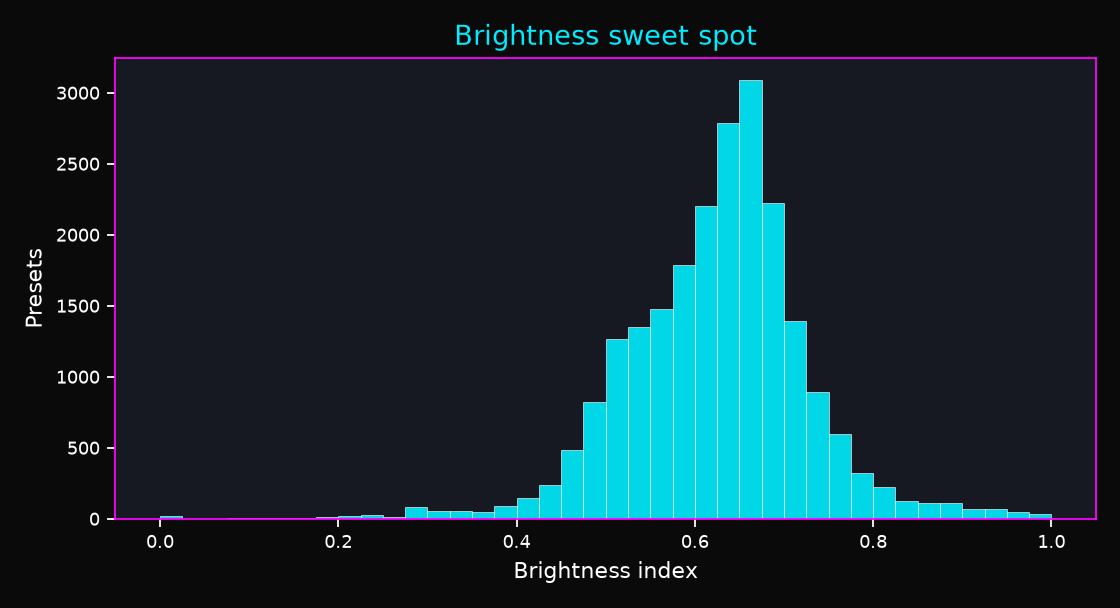
\includegraphics[width=\linewidth]{assets/fig_brightness_hist.png}%
    }{}
    \column{0.33\textwidth}
    \IfFileExists{assets/fig_brightness_by_game.png}{%
      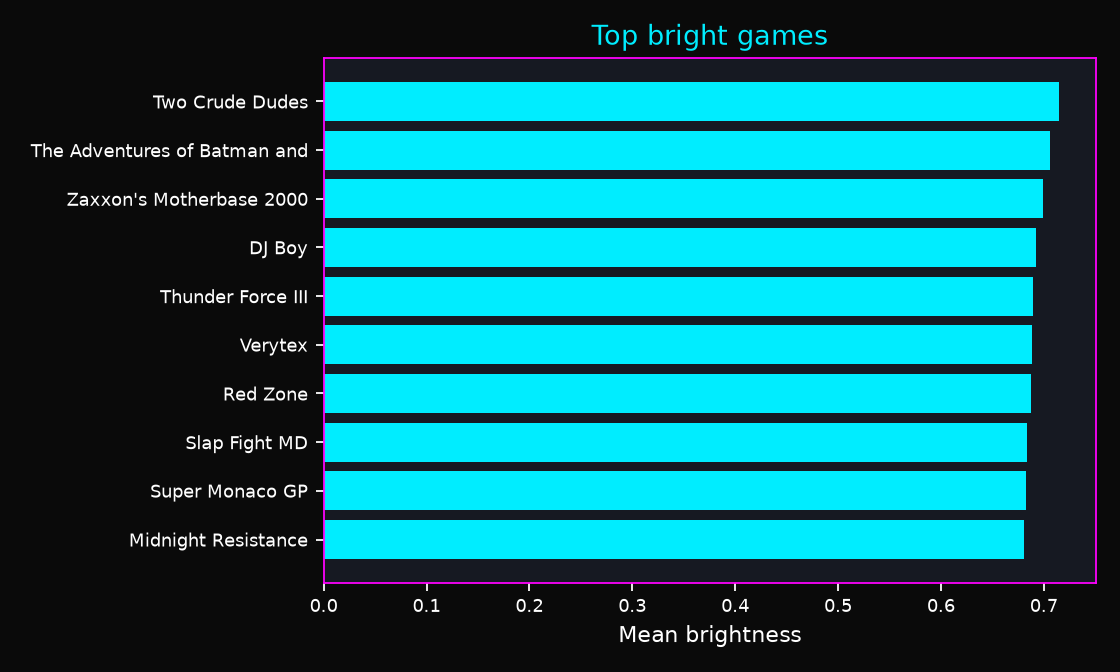
\includegraphics[width=\linewidth]{assets/fig_brightness_by_game.png}%
    }{}
    \column{0.33\textwidth}
    \IfFileExists{assets/fig_brightness_dark_games.png}{%
      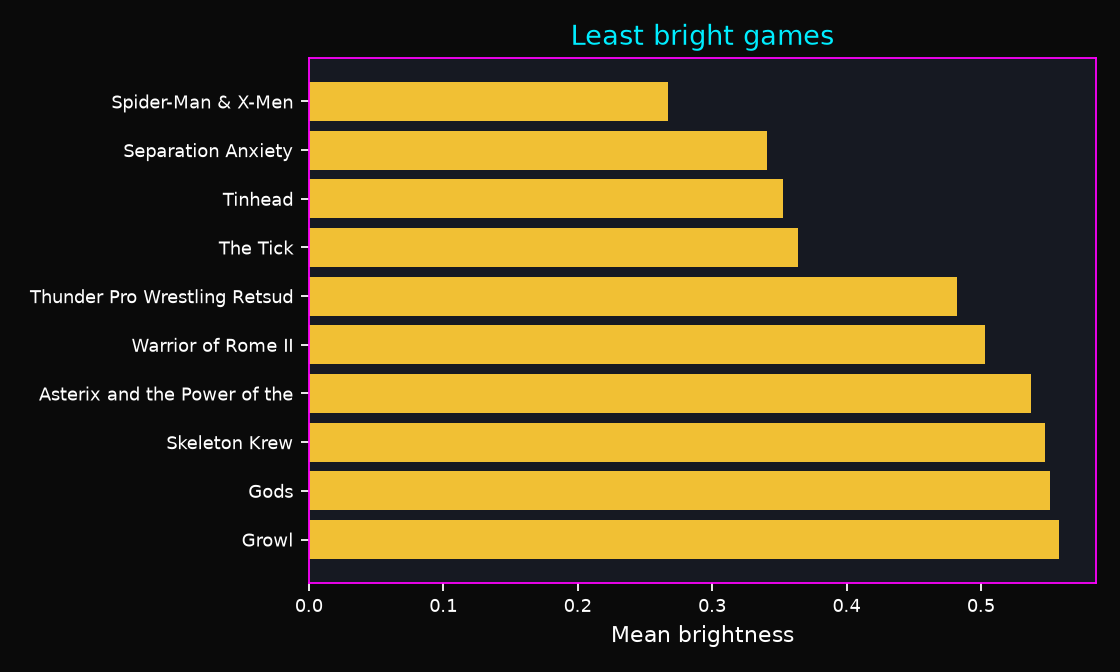
\includegraphics[width=\linewidth]{assets/fig_brightness_dark_games.png}%
    }{}
  \end{columns}
  \vspace{2mm}
  {\small Brightness from TL, attack, and multipliers --- presence on small TVs. Mid--high is the norm; a few titles stay deliberately darker.}
\end{frame}

%---------------------------------------------------------------------
\begin{frame}{GEMS --- the American sound driver}
  \begin{columns}[T,onlytextwidth]
    \column{0.48\textwidth}
    \textbf{GEMS} (Genesis Editor for Music and Sound): Sega of America's official tool (mid-1990s).
    \begin{itemize}
      \item Lowered the barrier to YM2612 programming
      \item Controversial: templates vs craft?
      \item In our corpus: a \textbf{tool variable}, not just a style label
    \end{itemize}
    \column{0.48\textwidth}
    \IfFileExists{assets/gems-interface.png}{%
      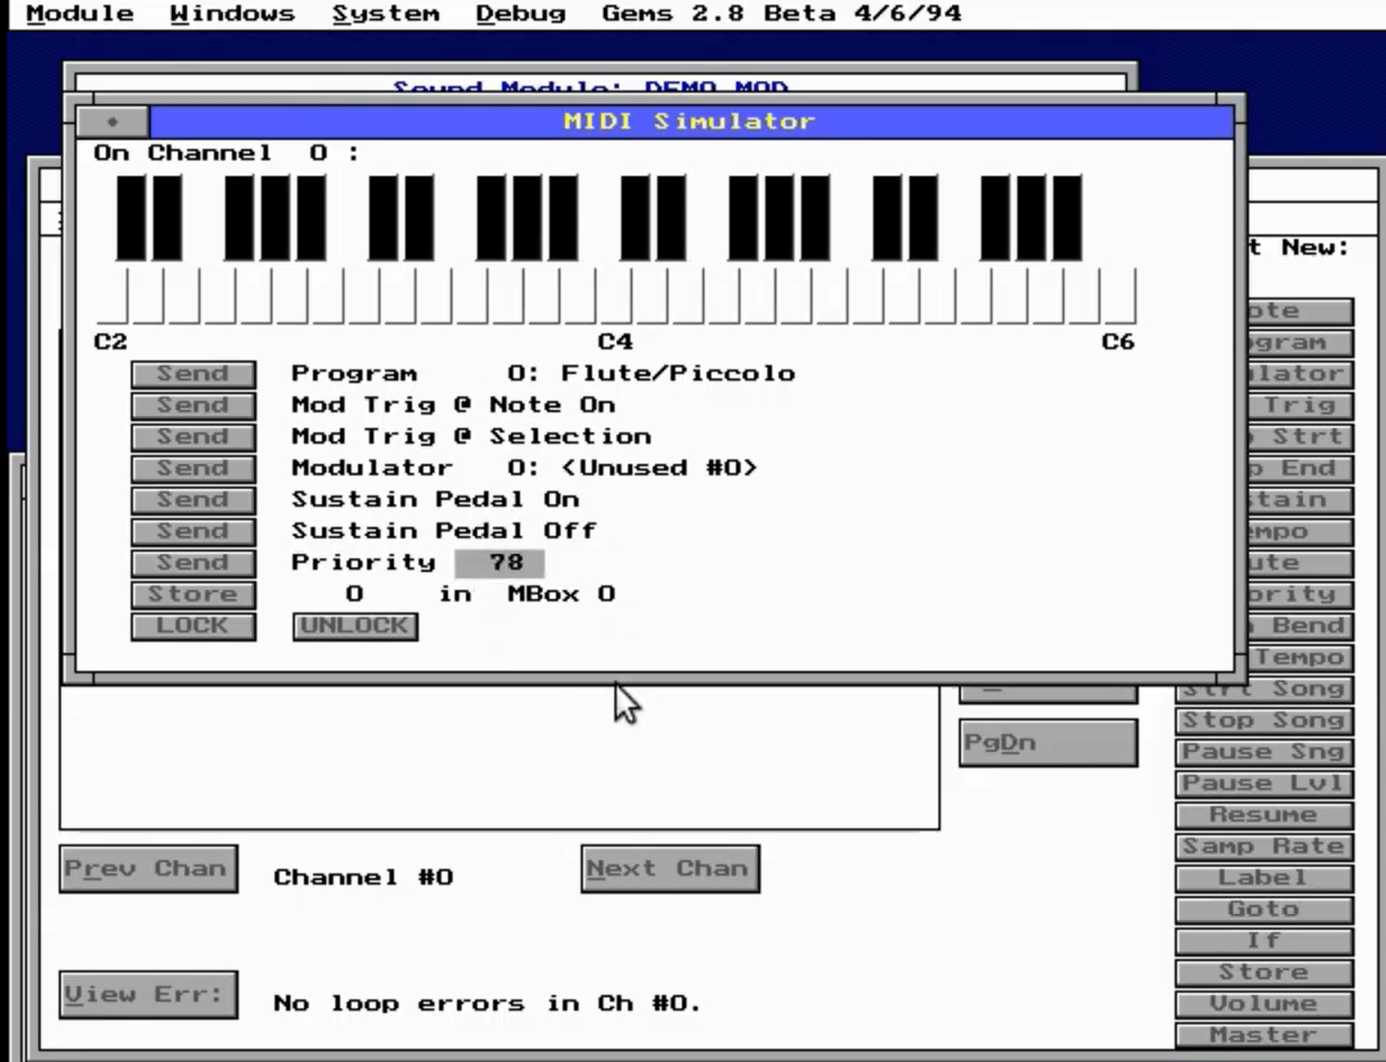
\includegraphics[width=\linewidth,height=0.55\textheight,keepaspectratio]{assets/gems-interface.png}%
    }{}
  \end{columns}
\end{frame}

%---------------------------------------------------------------------
\begin{frame}{GEMS in practice --- a concrete contrast}
  \begin{columns}[c,onlytextwidth]
    \column{0.55\textwidth}
    \IfFileExists{assets/fig_gems_case.png}{%
      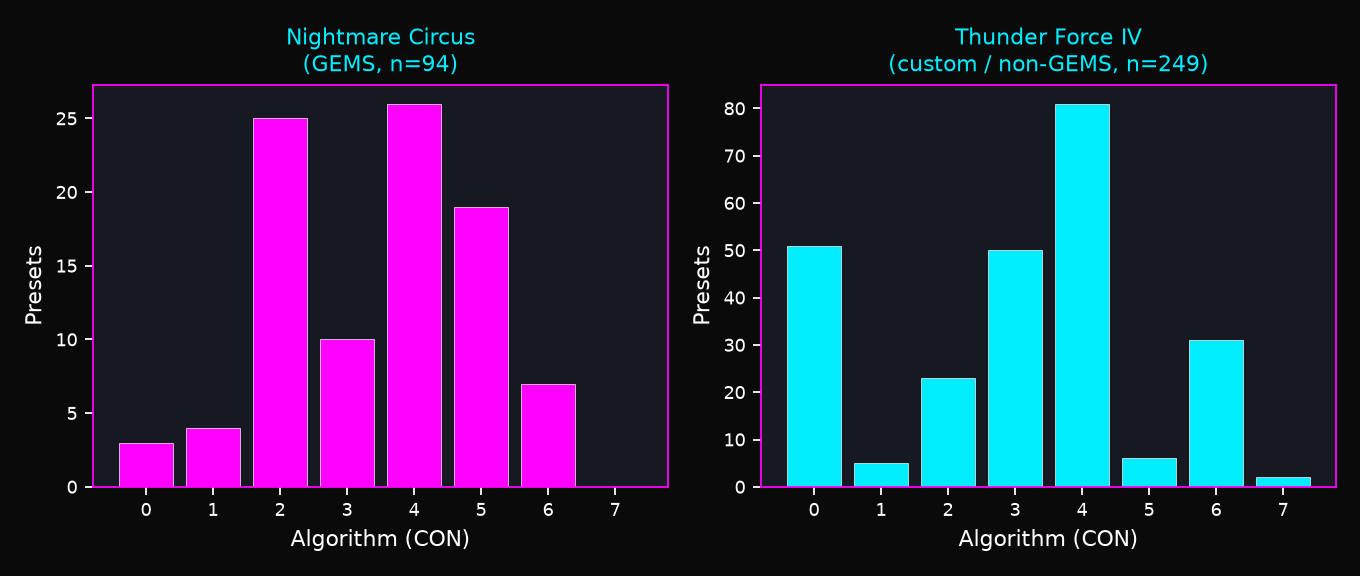
\includegraphics[width=\linewidth,height=0.48\textheight,keepaspectratio]{assets/fig_gems_case.png}%
    }{}
    \column{0.42\textwidth}
    \begin{itemize}
      \item \textbf{Nightmare Circus} (GEMS): shared tool ecosystem
      \item \textbf{Thunder Force~IV} (non-GEMS): broader CON spread
    \end{itemize}
    {\scriptsize Not worse vs better --- different industrial conditions.}
  \end{columns}
  \livebox{L3+L4}{\textit{Nightmare Circus} vs \textit{Thunder Force IV}: VGM + preset each}
\end{frame}

%---------------------------------------------------------------------
\begin{frame}{Composing by region / tool}
  \begin{columns}[c,onlytextwidth]
    \column{0.48\textwidth}
    \IfFileExists{assets/fig_nationality.png}{%
      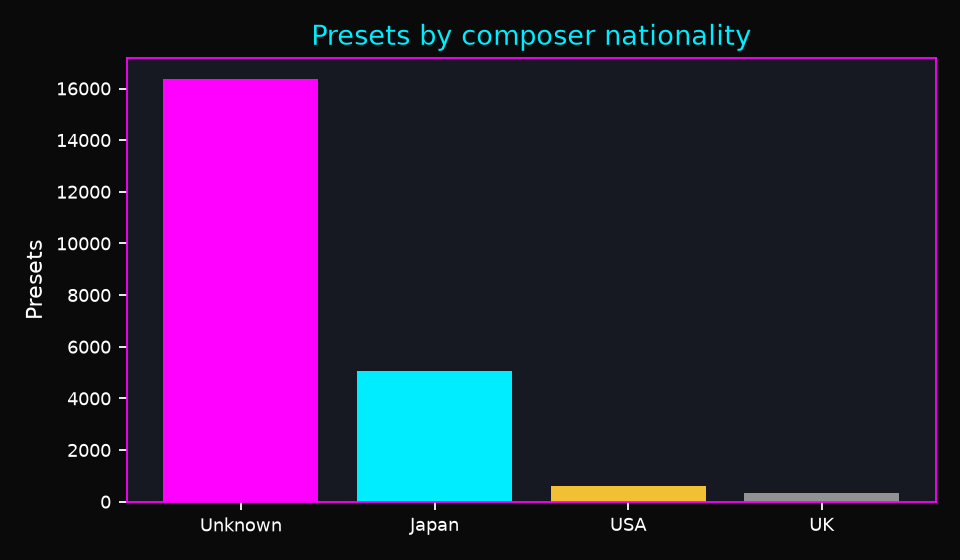
\includegraphics[width=\linewidth]{assets/fig_nationality.png}%
    }{}
    \column{0.48\textwidth}
    \IfFileExists{assets/fig_gems_brightness.png}{%
      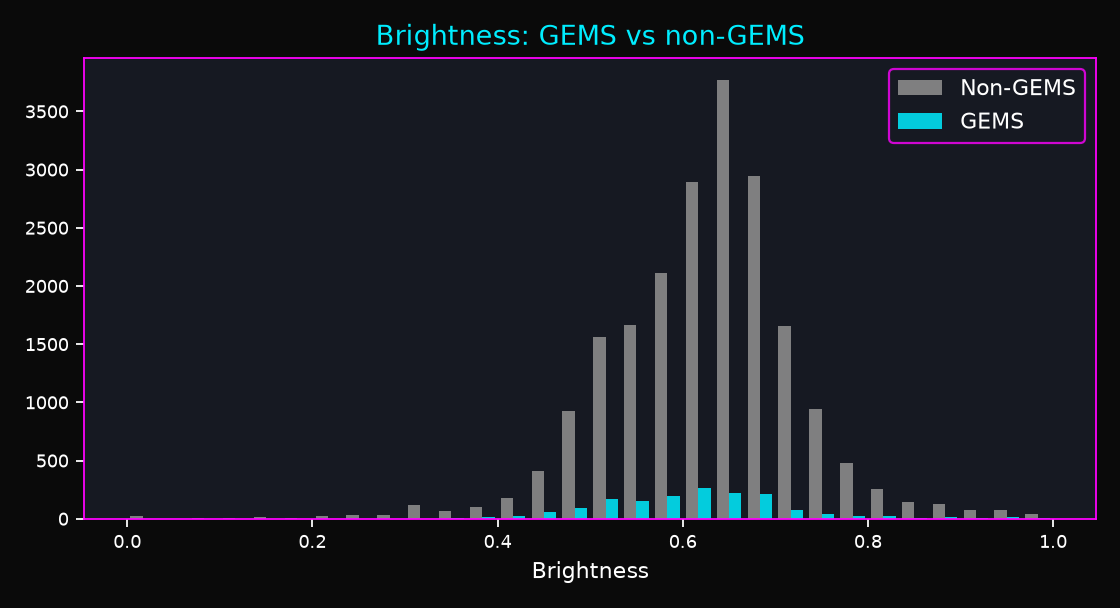
\includegraphics[width=\linewidth]{assets/fig_gems_brightness.png}%
    }{}
  \end{columns}
  \vspace{2mm}
  Japan / USA / UK as \textbf{hypotheses} about practice --- drivers, deadlines, and shared templates shape timbre as much as ``national style.''
\end{frame}

%---------------------------------------------------------------------
\begin{frame}{Composer signatures}
  \begin{columns}[T,onlytextwidth]
    \column{0.52\textwidth}
    \begin{itemize}
      \item \textbf{Yuzo Koshiro} --- house / techno energy into YM2612 (*Streets of Rage*)
      \item \textbf{Masato Nakamura} --- pop sensibility (*Sonic the Hedgehog*)
      \item Shared workhorse choices --- individuality in envelopes, brightness, game fingerprints
    \end{itemize}
    \column{0.45\textwidth}
    \IfFileExists{assets/fig_composers_brightness.png}{%
      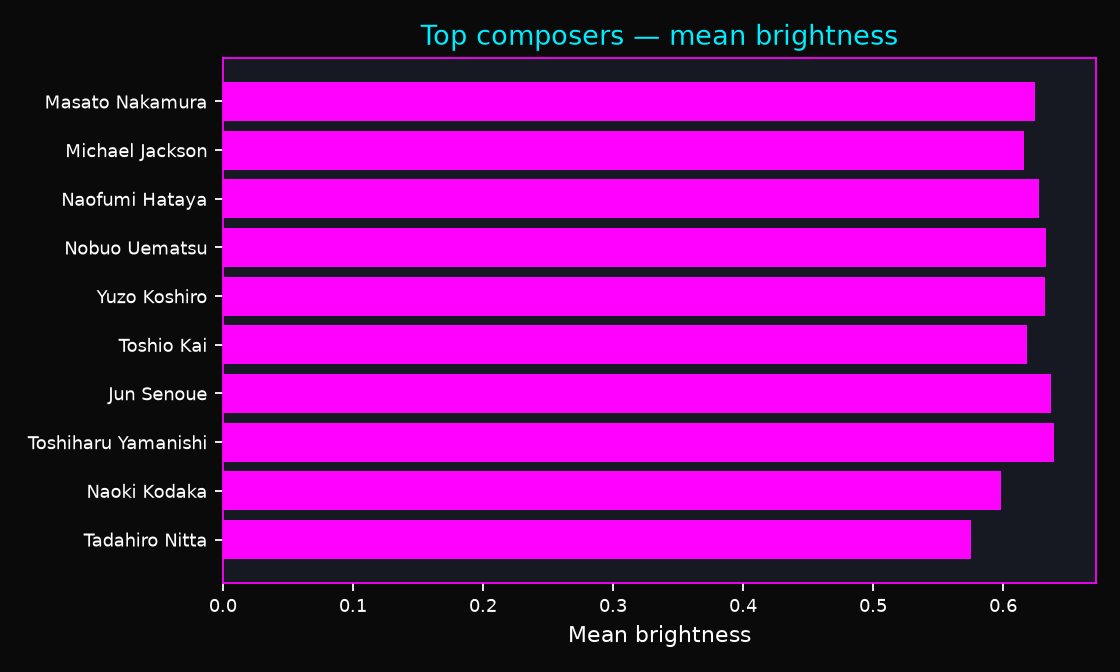
\includegraphics[width=\linewidth,height=0.42\textheight,keepaspectratio]{assets/fig_composers_brightness.png}%
    }{}
  \end{columns}
  \livebox{L1}{\textit{Streets of Rage} VGM $\rightarrow$ high-FL Koshiro preset (VIDEO~3 only if live fails)}
\end{frame}

%---------------------------------------------------------------------
\begin{frame}{More signatures --- Kodaka \& Uematsu}
  \begin{columns}[c,onlytextwidth]
    \column{0.55\textwidth}
    \IfFileExists{assets/fig_composers_compare.png}{%
      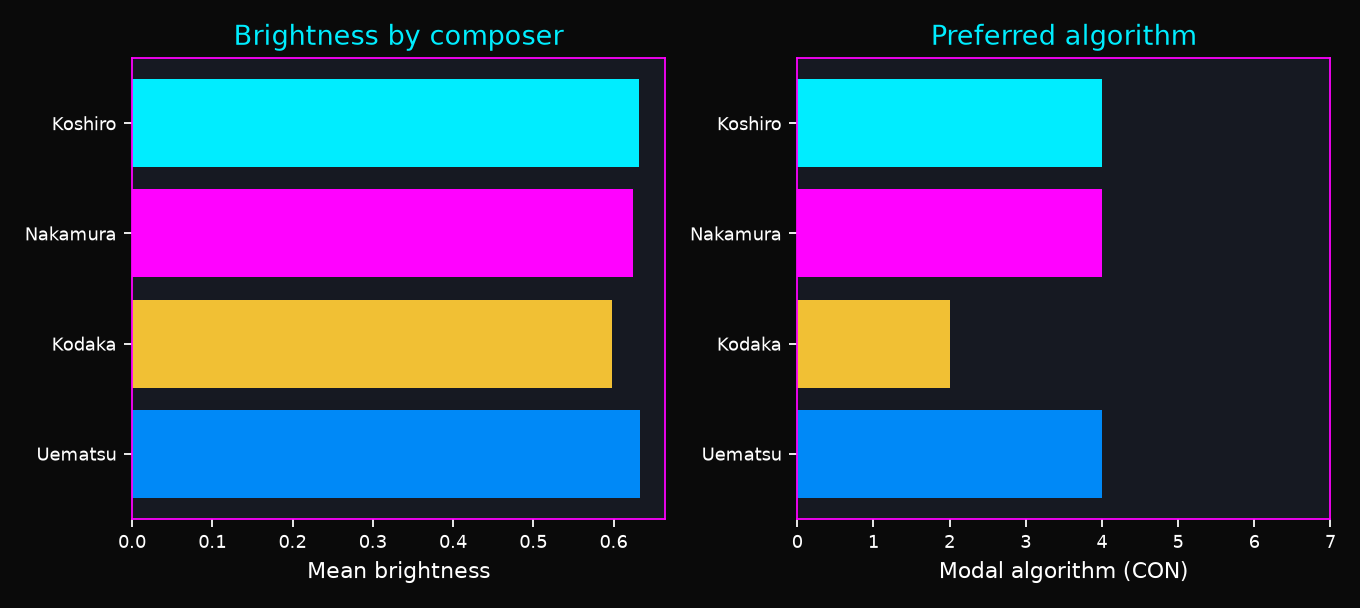
\includegraphics[width=\linewidth]{assets/fig_composers_compare.png}%
    }{}
    \column{0.42\textwidth}
    \begin{itemize}
      \item \textbf{Naoki Kodaka}: modal CON leans away from the Alg.~4 default --- more idiosyncratic routing
      \item \textbf{Nobuo Uematsu}: still near the workhorse grammar, with his own brightness / game palette
    \end{itemize}
    \vspace{2mm}
    {\small Convergence on tools of the chip $\neq$ identical sonic personalities.}
  \end{columns}
\end{frame}

%---------------------------------------------------------------------
\begin{frame}{Zooming out --- timbral neighbourhoods}
  \begin{columns}[c,onlytextwidth]
    \column{0.55\textwidth}
    \IfFileExists{assets/fig_embedding_clusters.png}{%
      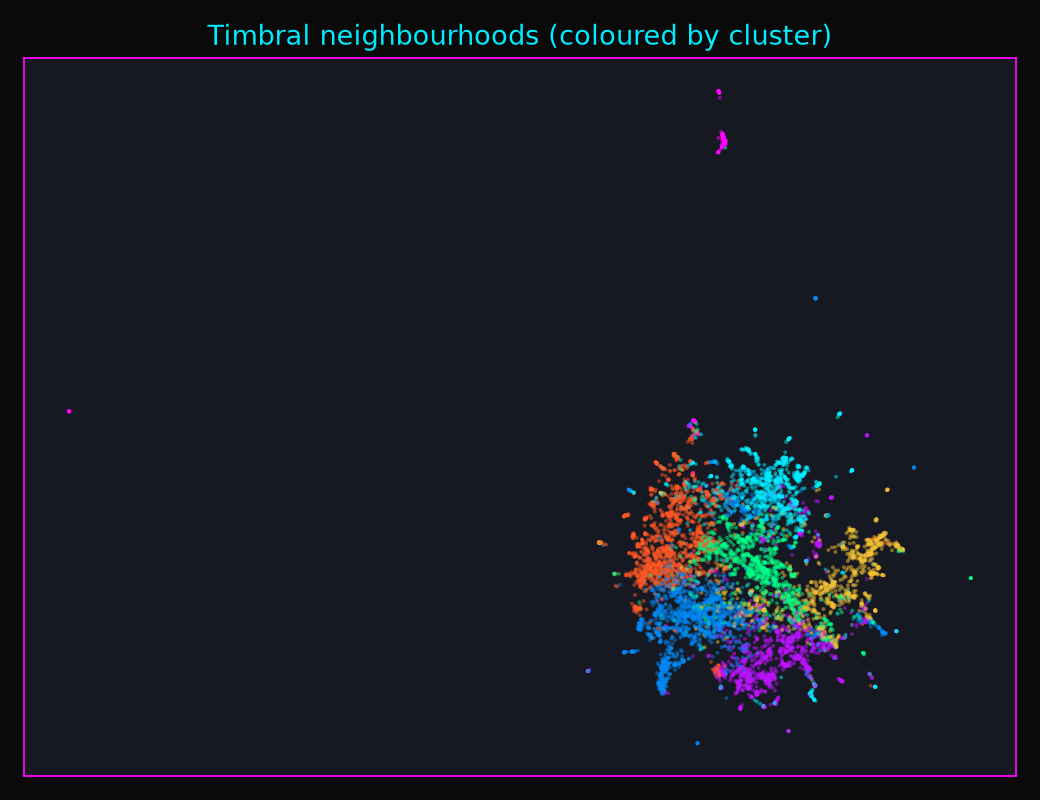
\includegraphics[width=\linewidth,height=0.62\textheight,keepaspectratio]{assets/fig_embedding_clusters.png}%
    }{}
    \column{0.42\textwidth}
    At full corpus scale, presets form \textbf{neighbourhoods}: similar voices land near each other.
    \vspace{2mm}
    Seven emergent ``sonic realms'' (from action neon to fantasy atmospheres) --- a map of practice, not a taxonomy imposed in advance.
    \vspace{2mm}
    {\scriptsize\textit{No ML tutorial here --- just the picture of the corpus.}}
  \end{columns}
\end{frame}

%---------------------------------------------------------------------
\begin{frame}{What the data does \emph{not} say}
  Honest limits keep the story scholarly:
  \begin{itemize}
    \item A preset is not a full score --- melodies, sequencing, and PCM drums live elsewhere
    \item Extraction inherits archive quirks (naming, completeness, scraping gaps)
    \item Clusters and maps are \textbf{exploratory}: invitations to listen, not closed taxonomies
    \item ``National style'' and ``GEMS sound'' are hypotheses under industrial constraints
  \end{itemize}
  \vspace{2mm}
  {\small The payoff: better questions about platform practice --- with sounds you can still hear.}
\end{frame}

%---------------------------------------------------------------------
\begin{frame}{Why this matters --- and open tools}
  \begin{itemize}
    \item Presets are evidence of \textbf{shared timbral practice} on a platform
    \item Extraction + exploratory analysis make composer, region, and tool differences discussable with data
    \item Method is open: code, documentation, and notebooks for reuse
  \end{itemize}
  \vspace{2mm}
  \begin{block}{Listen \& explore}
    \textbf{DAFMExplorer} --- interactive map, real-time YM2612 playback, filters.\\
    {\small\url{https://dafm-explorer.vercel.app/}}\\[1mm]
    {\scriptsize Next: same approach for other FM families (e.g.\ YM2151, YMF262).}
  \end{block}
\end{frame}

%---------------------------------------------------------------------
\begin{frame}{Thanks --- questions welcome}
  \begin{columns}[c,onlytextwidth]
    \column{0.42\textwidth}
    \IfFileExists{assets/logo-kasser-synths.png}{%
      
\includegraphics[width=0.85\linewidth]{assets/logo-kasser-synths.png}%
    }{}
    \column{0.55\textwidth}
    \textbf{Abraham Casas} \& \textbf{Maria Cerro}\\
    Kasser Synths\\[3mm]
    {\small\url{https://www.kassersynths.com}}\\
    {\small\url{https://dafm-explorer.vercel.app/}}\\
    {\small\url{https://github.com/kassersynths/DAFMExplorer}}\\[4mm]
    {\large\color{kasserMagenta}Thank you --- Q\&A}
  \end{columns}
\end{frame}

\end{document}
